%!TEX TS-program = XeLaTeX
\documentclass[11pt]{article}

\usepackage{amssymb}
\usepackage{amsthm}
\usepackage{amsmath}
\usepackage{mathtools}

\usepackage{fancyhdr}
\usepackage{graphicx}
\usepackage[top=3cm, left=2cm, right=2cm, headheight = 90pt]{geometry}
\usepackage{xltxtra}
\usepackage[font=small,labelfont=bf]{caption}

%%%%%%%%%%%%%%    Language matters  %%%%

%\usepackage[latvian]{babel}
%\usepackage[L7x]{fontenc}
%\usepackage[utf8x]{inputenc}

%%%%%%%%%%%%%%%%%%%%%%%%%%%%%%%%%%%7%%%%%

%%%%%%%%%%%%%%%%%%%%%%%%%%%       DO NOT EDIT         %%%%%%%%%%%%%%%%%%
%\usepackage{space}
%\renewcommand{\headrulewidth}{1pt}
%\fancyhead[L]{\includegraphics[width=3cm]{pictures/logo}}
%\fancyhead[R]{\raisebox{3ex}{\fbox{Language: \bf \lang}}}
\fancyhead[C]{{\Large\bf Induction - Problems}\\ \date}

\renewcommand{\theenumi}{\alph{enumi}}
%\newcommand{\problem}[1]{\paragraph{Problem #1.}}%<--------------- TRANSLATE THE WORD "Problem".
\fancyfoot[CE,CO]{}  % this is to remove page numbers (as you might want for single page docs)

\def\leq{\leqslant}
\def\geq{\geqslant}
\def\N{\mathbb N}
\def\R{\mathbb R}
\def\Z{\mathbb Z}
\DeclarePairedDelimiter\set\{\}
\newcommand{\?}{\stackrel{?}{=}}

%%%%%%%%%%%%%%%%%%%%%%%%%%%%%%%%%%%%%%%%%%%%%%%%%%%%%%%%%%%%%%%%%%%%%%%%%


%%% Language name in english %%%%%%%%%
\def\lang{Latvian}

%\def\lang{Lithuanian}

%%%%%%%%%%%%%%%%%%%%%%%%%%%%% TRANSLATE HERE %%%%%%%%%%%%%%%%%%%%%%%%%%%%%%%%%%

%\def\date{2018. gada 18. jūnijs}
%\def\notes{}


%%%%%%%%%%%%%%%%%%%%%%%%%%%%%%%%%%%%%%%%%%%%%%%%%%%%%%%%%%%%%%%%%%%%%%%%%%%%%%%

\def\prob{}

%%%%%%%%%%%%%%%%%%%%%%%%%%%%%%%%%%%%%%%%%%%%%%%%%%%%%%%%

\theoremstyle{definition}
\newtheorem{problem}{\prob}

\pagestyle{fancy}



\begin{document}
%\thispagestyle{fancy}
\noindent 
%\emph{\notes}

%1
\begin{problem}
\textit{[Grasshopper induction]}
An immortal grasshopper sits on a first step of an infinite ladder. This grasshopper is capable to harness the energy of the universe at a rate that allows it to jump to next step of a ladder every minute. 

Prove that the grasshopper will be able to reach its favourite star no matter how far it is! 
\end{problem}
%

%2
\begin{problem}
\textit{[Caterpillar induction]}
A very long (infinite) caterpillar has arrived at this infinite ladder and managed to raise its head and first legs to the first two steps. It knows that if it has a firm grip on first $k$ steps, then it can pull itself up and reach step $k+1$. 

Prove that it can also reach grasshoppers favourite star!
\end{problem}
%

%3
\begin{problem}
\textit{[Triangular numbers]}
A number $T$ is \textit{triangular} if it can make a triangular dot pattern. First triangular numbers are:
\begin{center}
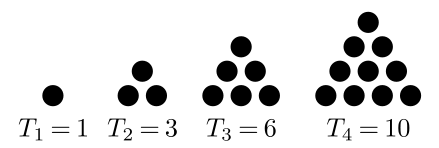
\includegraphics[width=5cm]{Triangular_numbers.png}
\captionof{figure}{First triangular numbers}
\label{fig:TriangularNumbers}
\end{center}

Prove that $T_n=\frac{n(n+1)}{2}$!
\end{problem}
%

%4
\begin{problem}
\textit{[Waterworks]}
There are $64$ glasses on a table, each with a different amount of water in it. Peter can take any two glasses and pour water from one to another until the amounts in these two glasses are equal.

Prove that Peter can reach a state where all the glasses on the table hold the same amount of water!
\end{problem}
%


%5
\begin{problem}
\textit{[Onewayland]}
In Onewayland every town is connected to each other by a one way road. 

Prove that there is a town from which you can travel to any other town in Onewayland!
\end{problem}
%


%6
\begin{problem}
\textit{[Another Onewayland]}
In this Onewayland some towns is connected to each other by a one way road (and there are no disconnected parts). It is also known that, for every town, number of roads leading into it equals number of roads going out of it.

Prove that it is possible to travel between any two towns in this Onewayland!
\end{problem}
%

%7
\begin{problem}
\textit{[One more Onewayland]}
We are again in Onewayland, where every town is connected to each other by a one way road. We know that there are at least $3$ towns here.

Prove that it is possible to change direction of no more than one road so that after the change it will be possible to travel between any two towns!
\end{problem}
%

%8
\begin{problem}
\textit{[Corner tiling of square]}
Someone removed one cell from a $128\times128$ square. 

Prove that is possible to tile the remaining cells with "3-cell corner" figures!
\begin{center}
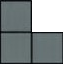
\includegraphics[width=1cm]{corner.png}
\captionof{figure}{3-cell corner}
\label{fig:Coner}
\end{center}
\end{problem}
%

%9
\begin{problem}
\textit{[Foxy problem]}
$100$ rabbits found some berries in the wood. Youngest managed to get $1$ berry, second youngest - $2$ berries, third - $4$ and so on, with eldest getting $2^{99}$ berries. A fox came up and suggested a "fairer" distribution - the fox repeatedly choose two rabbits and re-distribute the berries they have together evenly between the two rabbits. If the total number the two rabbits have is odd, the fox would eat one berry and distribute berries evenly between the two. 
What is the maximum amount of berries fox can eat following these rules?
\end{problem}
%

%10
\begin{problem}
\textit{[Cliques again!]}
There are $n$ people in a group some of whom are pairwise friends. Lets denote number of friends of person $i$ within this group by $d_i$. Prove that there are at least 
$\sum_{i=1}^{n}{\frac{1}{d_i +1}}$
people in this group none of whom are friends with each other.
\end{problem}
%

%11 IMO2006 SLC1
\begin{problem}
\textit{[Lamp flicking]}

We have $n \ge 2$ lamps $L_1, \dots, L_n$ in a row, each of them being either on or off. Every second we simultaneously modify the state of each lamp as follows:
\begin {itemize}
\item if the lamp $L_i$ and its neighbours (only one neighbour for $i = 1$ or $i = n$, two neighbours for other $i$) are in the same state, then $L_i$ is switched off;
\item otherwise, $L_i$ is switched on.
\end {itemize}
Initially all the lamps are off except the leftmost one which is on.
\begin {enumerate}
\item Prove that there are infinitely  many integers $n$ for which  all the lamps will eventually be off.
\item Prove that there are infinitely many integers $n$ for which the lamps will never be all off.
\end {enumerate}

\end{problem}
%

%12 IMO2005 SLC5
\begin{problem}
\textit{[Coin flipping]}

There are $n$ coins, each with one side white and the other side black, aligned in a row so that their white sides are up. In each step, if possible, we choose a coin with the white side up (but not one of outermost coins), remove it and flip the closest coin to the left and the closest coin to the right of it. Prove that one can achieve the state with only two coins remaining if and only if $n − 1$ is not divisible by $3$.


\end{problem}
%
\end{document}
